\documentclass{article}

% if you need to pass options to natbib, use, e.g.:
%     \PassOptionsToPackage{numbers, compress}{natbib}
% before loading neurips_2022

% ready for submission
\usepackage[preprint]{neurips_2022}

% to compile a preprint version, e.g., for submission to arXiv, add add the
% [preprint] option:
%     \usepackage[preprint]{neurips_2020}

% to compile a camera-ready version, add the [final] option, e.g.:
%     \usepackage[final]{neurips_2020}

% to avoid loading the natbib package, add option nonatbib:
%\usepackage[nonatbib]{neurips_2020}
\usepackage[utf8]{inputenc} % allow utf-8 input
\usepackage[T1]{fontenc}    % use 8-bit T1 fonts
\usepackage{hyperref}       % hyperlinks
\usepackage{url}            % simple URL typesetting
\usepackage{booktabs}       % professional-quality tables
\usepackage{amsfonts}       % blackboard math symbols
\usepackage{nicefrac}       % compact symbols for 1/2, etc.
\usepackage{microtype}      % microtypography


% Graphics and color
\usepackage{graphicx}
\usepackage{xcolor}

% References and Bibliography
\usepackage{url}
\usepackage{hyperref}
\hypersetup{
  colorlinks,
  linkcolor={black},
  citecolor={blue!50!black},
  urlcolor={blue!50!black}
}
\usepackage{cleveref}
\usepackage[numbered]{bookmark} % Fixes false PDF table of contents
\usepackage{natbib}
\setcitestyle{numbers,sort&compress,square,comma}
\usepackage{bibentry}
\nobibliography*

\title{Impact of most Common Food Categories on\\ Green House Gas Emissions}


\author{%
  Hanna Dettki\thanks{Equal contribution.} \\
  Department of Computer Science\\
  University of Tübingen\\
  \texttt{hanna.dettki@student.uni-tuebingen.de} \\
  \And
  Davide $^{*}$  \\
  Department of Computer Science\\
  University of Tübingen\\
  \texttt{@student.uni-tuebingen.de} \\
  % \AND
  % Coauthor \\
  % Affiliation \\
  % Address \\
  % \texttt{email} \\
  % \And
  % Coauthor \\
  % Affiliation \\
  % Address \\
  % \texttt{email} \\
  % \And
  % Coauthor \\
  % Affiliation \\
  % Address \\
  % \texttt{email} \\
}

\begin{document}

\maketitle

\begin{abstract}
  some abstract
\end{abstract}

\section{Introduction}



\begin{figure}[h]
  \centering
  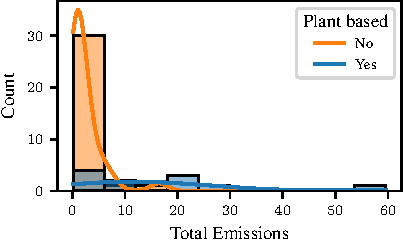
\includegraphics[width=0.5\textwidth]{figures/testplot.pdf}
  \caption{Some caption text.}
\end{figure}

\subsection{Research Question}



\section{Data}
\label{data}

\paragraph{Handling missing data}
We substituted  missing  data by taking the mean of the respecting feature. 
\subsection{Data Generating Process}
\label{dataGen}



\section{Analysis}
\label{analysis}
\subsection{Average Emissions for Plant-based and Animal-based Products}
\paragraph{Eutrophying emissions}
\paragraph{Accounting  for Nutritional Value}
\paragraph{Comparing Typical Diets}

\section{Conclusion}
\label{conclusion}


\section{Limitations}
\label{limitations}

\subsection{Citations within the text}


\subsection{Tables}



Note that publication-quality tables \emph{do not contain vertical rules.} We
strongly suggest the use of the \verb+booktabs+ package, which allows for
typesetting high-quality, professional tables:
\begin{center}
  \url{https://www.ctan.org/pkg/booktabs}
\end{center}
This package was used to typeset Table~\ref{sample-table}.

\begin{table}
  \caption{Sample table title}
  \label{sample-table}
  \centering
  \begin{tabular}{lll}
    \toprule
    \multicolumn{2}{c}{Part}                   \\
    \cmidrule(r){1-2}
    Name     & Description     & Size ($\mu$m) \\
    \midrule
    Dendrite & Input terminal  & $\sim$100     \\
    Axon     & Output terminal & $\sim$10      \\
    Soma     & Cell body       & up to $10^6$  \\
    \bottomrule
  \end{tabular}
\end{table}


\section*{Broader Impact}

Authors are required to include a statement of the broader impact of their work, including its ethical aspects and future societal consequences. 
Authors should discuss both positive and negative outcomes, if any. For instance, authors should discuss a) 
who may benefit from this research, b) who may be put at disadvantage from this research, c) what are the consequences of failure of the system, and d) whether the task/method leverages
biases in the data. If authors believe this is not applicable to them, authors can simply state this.

Use unnumbered first level headings for this section, which should go at the end of the paper. {\bf Note that this section does not count towards the eight pages of content that are allowed.}



\section*{Literature}

List of selected central research literature that the project is based on.


\begin{itemize}
  \item \bibentry{Ritchie2020}
  \item \bibentry{Michigan2021}
\end{itemize}

\subsection{Related Literature}
\begin{itemize}
  \item \bibentry{Pieper2020}
  \item \bibentry{Felix2021}
\end{itemize}


{\small
\bibliographystyle{unsrtnat}
\bibliography{../literature/references.bib}
}
\end{document}
